\documentclass[UTF8,a4paper,12pt]{ctexart} 
\usepackage{graphicx} 
\usepackage{amsmath} 
\usepackage{booktabs} 
\usepackage{geometry} 
\usepackage{listings} 
\usepackage{xcolor} 
\usepackage{subcaption}    % 并排子图 
\usepackage{placeins}      % 禁止浮动跨章节 
\usepackage{fancyhdr}      % 页眉页脚，消除右上角细数字标记 

% ========== 标题格式：section/subsection全部左对齐，大标题子标题对齐 ========== 
\ctexset{ 
	section={ 
		format={\Large\bfseries}, 
		number=\arabic{section}, 
		name={}, 
		aftername={\quad}, 
		beforeskip={1.5ex plus 0.2ex minus 0.2ex}, 
		afterskip={1.0ex plus 0.2ex minus 0.2ex} 
	}, 
	subsection={ 
		format={\large\bfseries}, 
		number=\arabic{section}.\arabic{subsection}, 
		name={}, 
		aftername={\quad}, 
		beforeskip={1.2ex plus 0.2ex minus 0.2ex}, 
		afterskip={0.8ex plus 0.2ex minus 0.2ex} 
	} 
} 

% ========== 页眉页脚：清除页眉多余细字体2、3标记，页码底部居中 ========== 
\pagestyle{plain} 
\fancyhf{} 
\cfoot{\thepage} 

\geometry{left=2.5cm,right=2.5cm, 
	top=2.5cm,bottom=2.5cm} 

% lstlisting Python代码样式 
\lstset{ 
	language=Python, 
	basicstyle=\ttfamily\small, 
	commentstyle=\color{gray}, 
	numbers=none, 
	frame=single, 
	breaklines=true 
} 

\title{ 
	基于光伏板结构线方向的机器人旋转角度视觉检测算法研究 
} 
\author{蔡依思} 
\date{\today} 
\begin{document} 
	
	\maketitle 
	
\begin{abstract}
	针对光伏板机器人旋转过程中角度难以直接获取的问题，本文提出一种基于光伏板结构线方向变化的视觉旋转角度检测方法。利用LSD直线检测提取光伏板结构线，通过分析结构线方向变化估计机器人旋转角度，并分别采用单方向累计和双方向跟踪两种方法进行实验比较。实验选取30$^\circ$、60$^\circ$、90$^\circ$、120$^\circ$、150$^\circ$和180$^\circ$六组旋转数据进行验证。结果表明，单方向方法在当前实验条件下具有较高的角度检测精度，平均绝对误差为0.073$^\circ$；双方向方法虽然角度误差略大，但能够通过A/B方向一致性误差对检测结果进行辅助可靠性评价。实验表明，基于光伏板结构线的视觉方法能够有效实现机器人旋转角度检测。
\end{abstract}
	
	
	\section{引言} 
	\subsection{研究背景} 
	
	光伏板清扫机器人在实际运行过程中需要频繁进行转向运动， 
	准确获取机器人旋转角度对于路径规划、定位以及自主导航具有重要意义。 
	
	传统机器人通常利用IMU、编码器等传感器获取姿态变化， 
	但视觉方法具有无需额外硬件、能够利用环境结构信息等优势。 
	
	本文研究对象为搭载摄像头的光伏板机器人。 
	实验数据来源于Blender仿真环境， 
	首先生成机器人视角视频，随后转换为鸟瞰视角图像进行视觉分析. 
	
	\vspace{12em} % 这里空3行，把背景文字和图片隔开，避免文字跨页跑到图片上方 
	
	\begin{figure}[htbp] 
		\centering 
		\begin{subfigure}{0.46\linewidth} 
			\centering 
			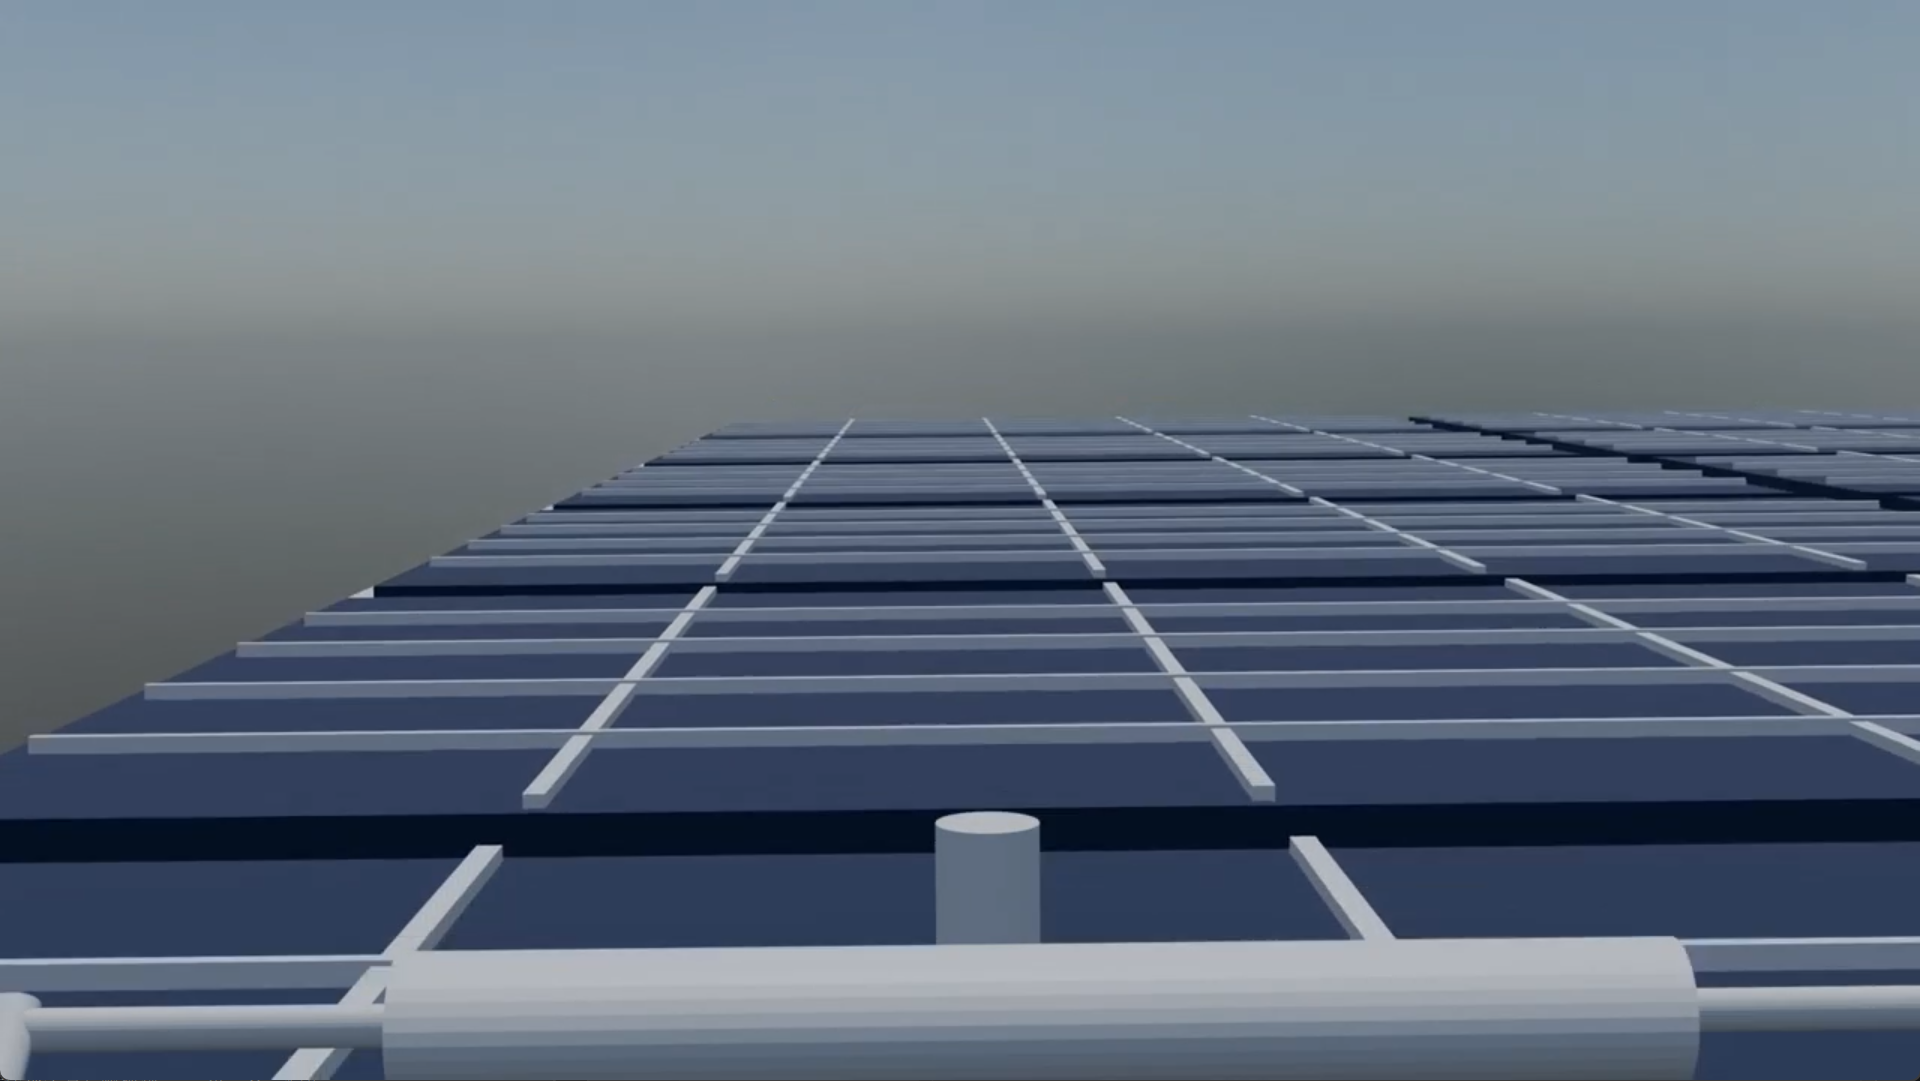
\includegraphics[width=\linewidth]{fig/original_view.png} 
			\caption{机器人原始车载倾斜视角} 
		\end{subfigure} 
		\hfill 
		\begin{subfigure}{0.46\linewidth} 
			\centering 
			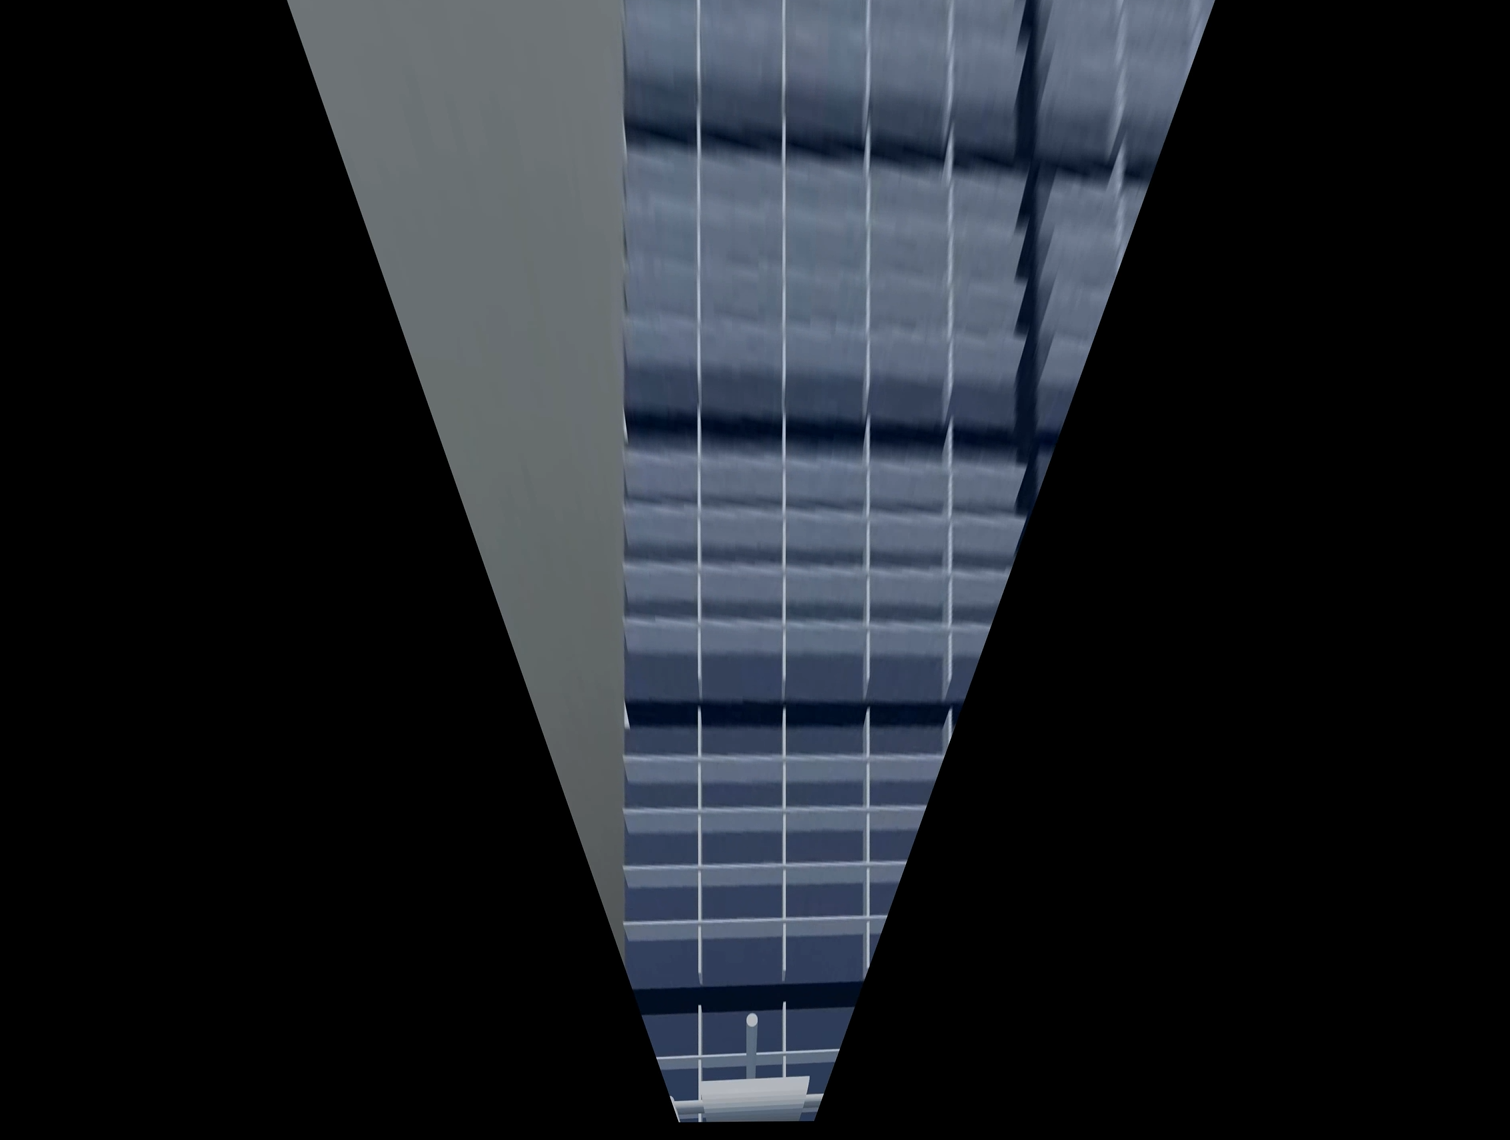
\includegraphics[width=\linewidth]{fig/bev_view.png} 
			\caption{透视变换后鸟瞰BEV视图} 
		\end{subfigure} 
		\caption{光伏机器人原始视角与鸟瞰变换视图对比} 
		\label{fig:view_compare} 
	\end{figure} 
	
	\subsection{研究目标} 
	本文主要研究以下问题： 
	\begin{itemize} 
		\item 如何利用光伏板结构线检测机器人旋转角度； 
		\item 单方向累计方法和双方向跟踪方法的检测效果； 
		\item 两种方法在角度精度、稳定性以及适用场景方面的差异。 
	\end{itemize} 
	
	其中，角度精度主要通过检测结果与真实旋转角度之间的误差进行评价； 
	稳定性主要分析算法在连续旋转过程中的方向跟踪情况； 
	适用场景则针对两种方法在不同检测需求下的应用特点进行讨论。 
	
	\FloatBarrier 
	
	
	
	\section{视觉旋转角度检测基础原理} 
	\subsection{机器人旋转与图像方向变化关系} 
	实验中光伏板在世界坐标系中保持静止， 
	而摄像机安装在机器人上。 
	
	因此机器人旋转会导致光伏板纹理方向在图像中发生变化。 
	
	其关系近似满足： 
	\begin{equation} 
		\Delta\theta_{\text{robot}} 
		\approx 
		-\Delta\theta_{\text{panel}} 
	\end{equation} 
	因此通过检测光伏板方向变化即可估计机器人旋转角度. 
	
	\subsection{LSD直线检测} 
	本文采用LSD(Line Segment Detector)检测光伏板中的结构线. 
	
	对于检测得到的线段： 
	\[ 
	(x_1,y_1),(x_2,y_2) 
	\] 
	
	其方向角计算为： 
	\begin{equation} 
		\theta= 
		\arctan 
		\frac{y_2-y_1}{x_2-x_1} 
	\end{equation} 
	
	由于直线不存在正反方向： 
	\begin{equation} 
		0^\circ\equiv180^\circ 
	\end{equation} 
	
	因此采用180度周期处理： 
	\begin{equation} 
		\Delta\theta= 
		\big((\theta_t-\theta_{t-1}+90) 
		\bmod 180\big)-90 
	\end{equation} 
	
	\begin{figure}[htbp!] 
		\centering 
		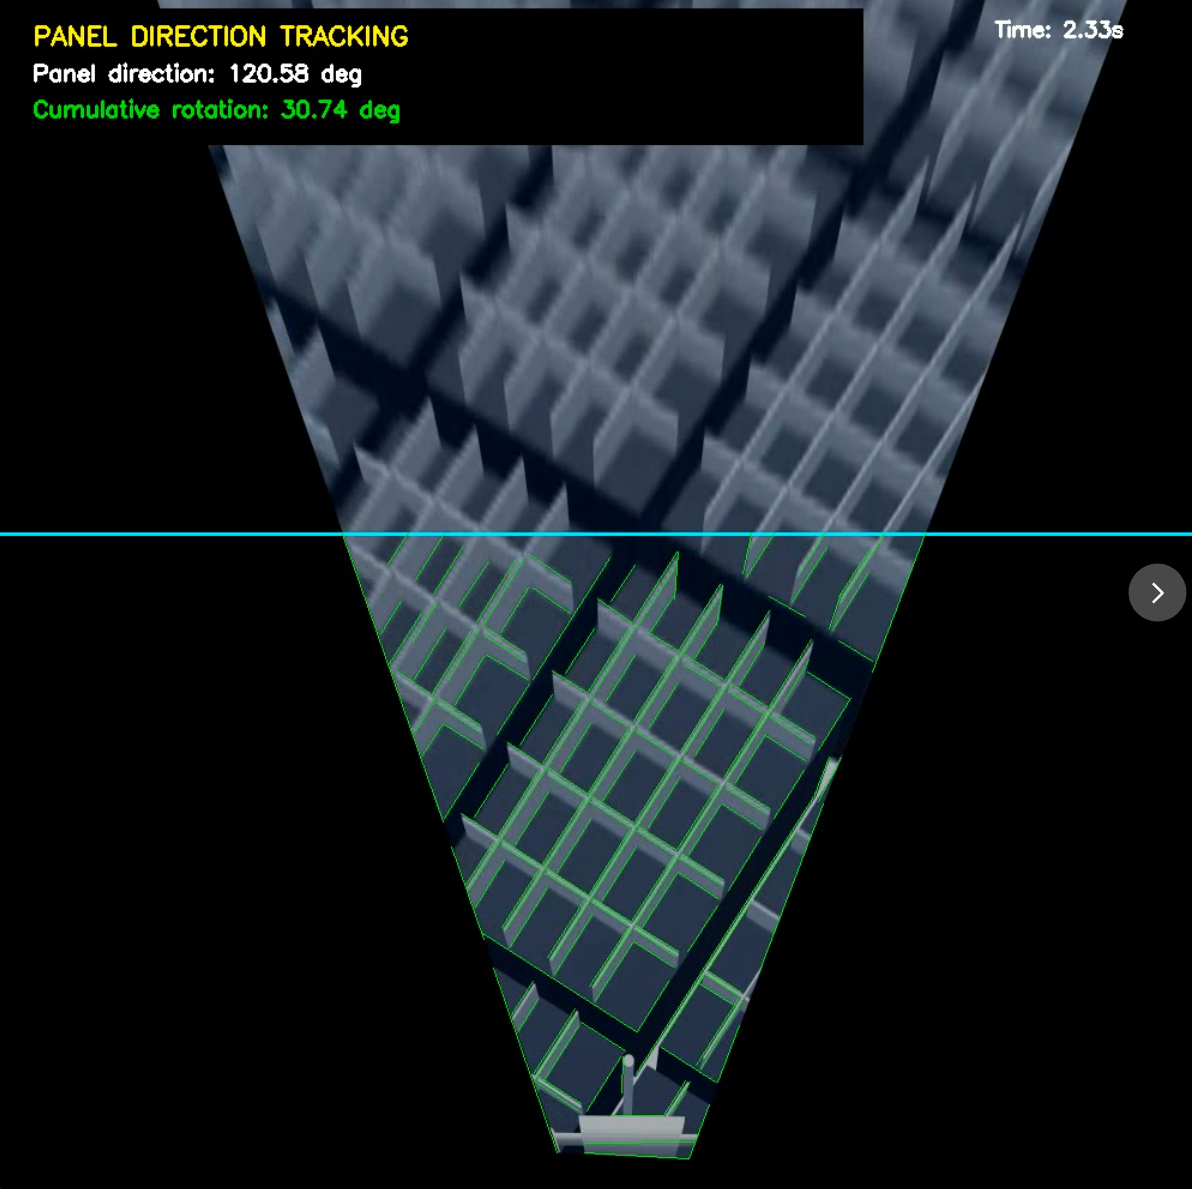
\includegraphics[width=0.75\linewidth]{fig/lsd_result.png} 
		\caption{LSD检测得到的光伏板结构线} 
	\end{figure} 
	
	\FloatBarrier 
	
	\section{单方向累计角度检测算法} 
	% ========== 3.1 核心代码（你的需求：代码放在算法思想前面） ========== 
	\subsection{核心算法代码} 
	\begin{lstlisting} 
		def angle_diff_180(a, b): 
		return (b - a + 90.0) % 180.0 - 90.0 
		
		# 每帧更新方向并累计旋转角度 
		if ok: 
		history.append(direction) 
		if len(history) > ANGLE_SMOOTH_WINDOW: 
		history.pop(0) 
		smoothed = circular_mean_180( 
		history, 
		np.ones(len(history)) 
		) 
		if prev is not None: 
		cumulative += angle_diff_180( 
		prev, 
		smoothed 
		) 
		prev = smoothed 
	\end{lstlisting} 
	
	该代码首先利用\texttt{Circular Mean}对最近5帧方向进行平滑，再通过$180^\circ$周期角度差计算相邻帧方向变化，并将每一帧的方向变化累加，从而获得机器人累计旋转角度。 
	
	\subsection{算法思想} 
	单方向算法首先利用LSD获取图像中的所有线段， 
	然后统计线段方向分布， 
	选择其中最明显的方向作为主方向. 
	
	算法流程如下： 
	\begin{figure}[htbp!] 
		\centering 
		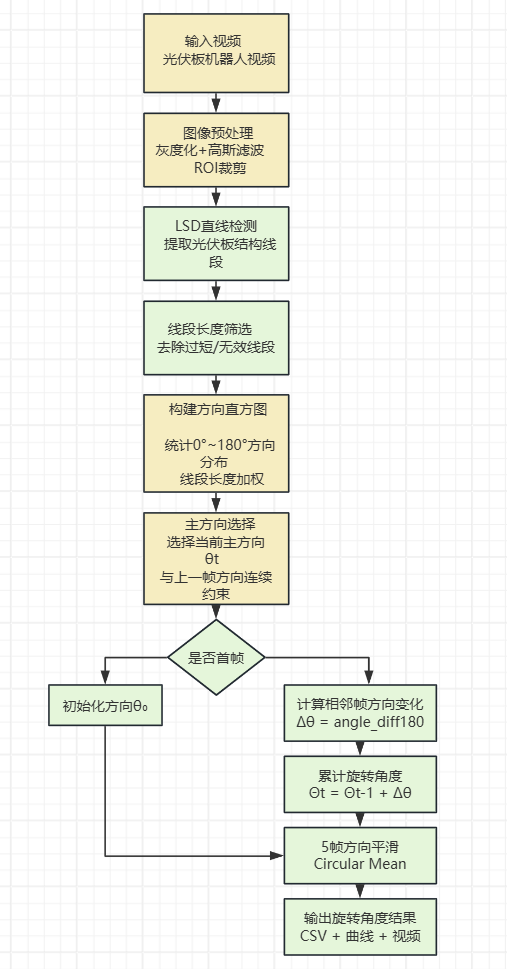
\includegraphics[width=0.65\linewidth]{fig/single_algorithm_flow.png} 
		\caption{单方向累计角度算法流程} 
	\end{figure} 
	
	主要步骤： 
	\begin{enumerate} 
		\item LSD检测线段； 
		\item 计算所有线段方向； 
		\item 建立方向直方图； 
		\item 选择主方向； 
		\item 进行时间连续跟踪； 
		\item 累计方向变化得到旋转角度。 
	\end{enumerate} 
	
	累计角度计算： 
	\begin{equation} 
		\Theta= 
		\sum_{t=1}^{N} 
		\Delta\theta_t 
	\end{equation} 
	
	\FloatBarrier 
	
	\section{双方向跟踪角度检测算法} 
	% ==========4.1核心代码，4.2算法思想 ========== 
	\subsection{核心算法代码} 
	\begin{lstlisting} 
		# A、B 两个方向分别累计旋转角度 
		if current_a is not None and prev_a is not None: 
		delta_a = angle_diff(prev_a, current_a) 
		cumulative_a += delta_a 
		if current_b is not None and prev_b is not None: 
		delta_b = angle_diff(prev_b, current_b) 
		cumulative_b += delta_b 
		
		# A/B 两个方向进行平均融合 
		mean_rotation = (cumulative_a + cumulative_b) / 2.0 
		
		# 计算两个方向累计结果的一致性误差 
		rotation_difference = abs(cumulative_a - cumulative_b) 
	\end{lstlisting} 
	
	该代码分别对A、B两个方向的帧间角度变化进行计算并累加，得到两个方向的累计旋转角度，再对A、B两个方向的累计结果进行平均融合，从而获得最终机器人旋转角度，同时通过计算两方向累计角度之差，对双方向检测结果的一致性进行评价。 
	
	\subsection{算法思想} 
	光伏板通常具有两组互相垂直的结构线： 
	\[ 
	|\theta_A-\theta_B|\approx90^\circ 
	\] 
	因此本文进一步设计双方向跟踪算法， 
	同时跟踪A、B两个方向. 
	
	流程： 
	\begin{figure}[htbp!] 
		\centering 
		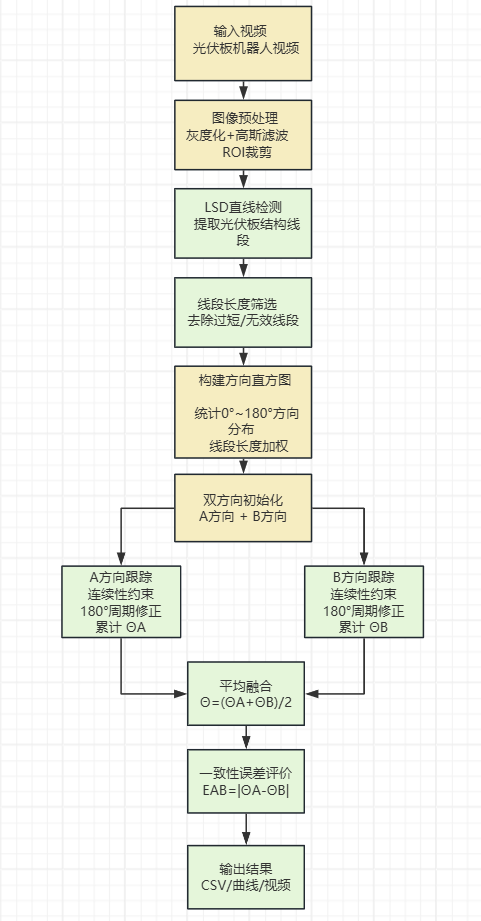
\includegraphics[width=0.65\linewidth]{fig/double_algorithm_flow.png} 
		\caption{双方向跟踪算法流程} 
	\end{figure} 
	
	A方向累计： 
	\begin{equation} 
		\Theta_A= 
		\sum\Delta\theta_A 
	\end{equation} 
	
	B方向累计： 
	\begin{equation} 
		\Theta_B= 
		\sum\Delta\theta_B 
	\end{equation} 
	
	最终结果： 
	\begin{equation} 
		\Theta= 
		\frac{\Theta_A+\Theta_B}{2} 
	\end{equation} 
	
	同时定义一致性误差： 
	\begin{equation} 
		E_{AB} 
		= 
		|\Theta_A-\Theta_B| 
	\end{equation} 
	
	由于A、B两个方向来源于同一光伏板结构， 
	理论上二者应具有相同的旋转变化趋势。 
	因此，当两个方向累计结果接近时， 
	说明当前方向检测具有较高一致性。 
	
	反之，如果A/B结果差异较大， 
	说明可能存在结构线检测不足、方向匹配错误或图像纹理变化等问题。 
	因此，A/B差值可以作为算法输出结果的可靠性评价指标。 
	
	 
	
	\section{实验设计} 
	\subsection{实验环境} 
	实验视频均由Blender生成. 
	
	\begin{table}[!htb] 
		\centering 
		\caption{实验视频参数} 
		\begin{tabular}{cccc} 
			\toprule 
			旋转角度 & FPS & 总帧数 & 时间(s)\\ 
			\midrule 
			30$^\circ$ &30&50&1.67\\ 
			60$^\circ$ &30&112&3.73\\ 
			90$^\circ$ &30&176&5.87\\ 
			120$^\circ$&30&238&7.93\\ 
			150$^\circ$&30&304&10.13\\ 
			180$^\circ$&24&300&12.50\\ 
			\bottomrule 
		\end{tabular} 
	\end{table} 
	
	所有实验采用： 
	\begin{itemize} 
		\item 相同ROI区域； 
		\item 相同LSD参数； 
		\item 相同方向周期处理方法。 
	\end{itemize} 
	
	\subsection{评价指标} 
	
	本文主要采用角度误差和A/B一致性误差评价算法性能。 
	
	角度绝对误差定义为： 
	\begin{equation} 
		E=|\Theta_{\text{det}}-\Theta_{\text{true}}|
	\end{equation} 
	
	其中，$\Theta_{\text{det}}$为算法检测结果， 
	$\Theta_{\text{true}}$为Blender设定的真实旋转角度。 
	
	对于双方向算法，进一步采用A/B一致性误差： 
	\begin{equation} 
		E_{AB}=|\Theta_A-\Theta_B|
	\end{equation} 
	
	该指标用于反映两个方向检测结果的一致程度， 
	不直接代表真实角度误差。 
	
	\subsection{双方向一致性误差分析} 
	
	双方向算法同时利用A、B两组结构线进行角度估计。 
	由于两组结构线属于同一光伏板结构， 
	机器人旋转时理论上应产生相同的角度变化。 
	
	因此，当$E_{AB}$较小时， 
	说明A、B两个方向得到的结果较为一致； 
	当$E_{AB}$增大时， 
	则可能存在某一方向检测不稳定的情况。 
	
	该指标不能代替真实角度误差， 
	但可以在缺少真实角度参考的实际应用中， 
	作为判断当前检测结果是否稳定的辅助依据。 
	
	\FloatBarrier 
	
	\section{实验结果} 
	\subsection{单方向算法结果} 
	\begin{figure}[htbp!] 
		\centering 
		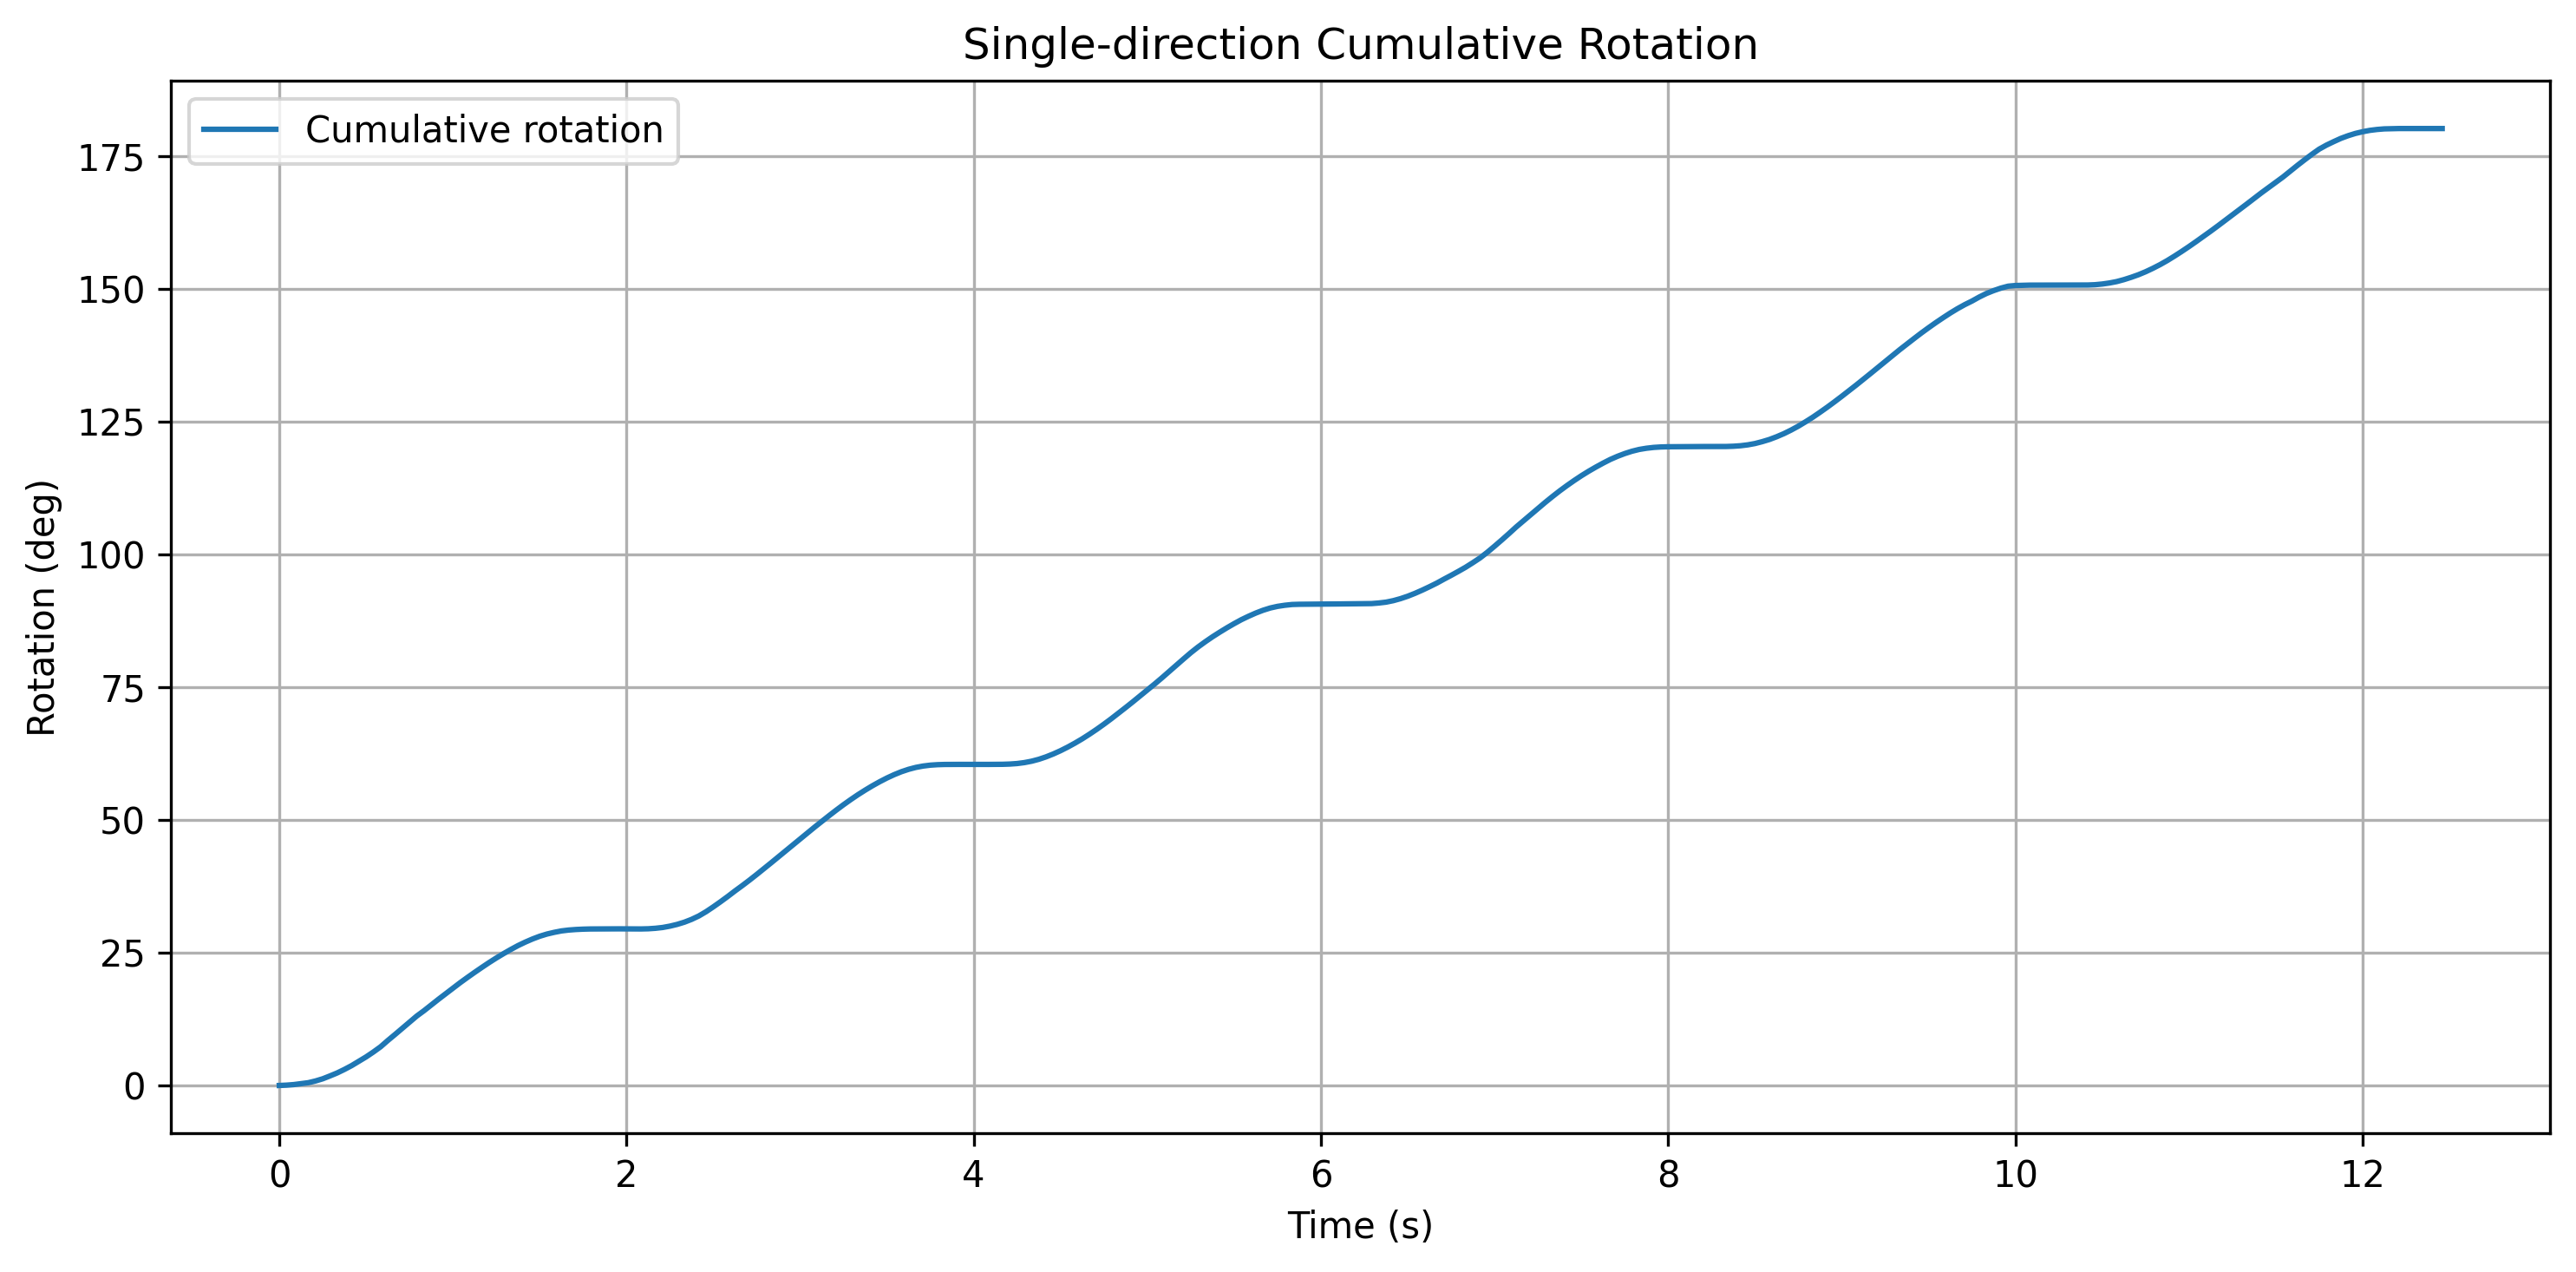
\includegraphics[width=0.8\linewidth]{fig/single_curve.png} 
		\caption{单方向算法累计旋转角度曲线} 
	\end{figure} 
	
	\begin{table}[!htb] 
		\centering 
		\caption{单方向算法检测结果} 
		\begin{tabular}{cccc} 
			\toprule 
			参考角度 & 检测角度 &误差\\ 
			\midrule 
			30&29.993&0.007\\ 
			60&60.126&0.126\\ 
			90&89.882&0.118\\ 
			120&119.951&0.049\\ 
			150&150.094&0.094\\ 
			180&179.956&0.044\\ 
			\bottomrule 
		\end{tabular} 
	\end{table} 
	
	实验结果表明， 
	单方向算法能够稳定跟踪光伏板主方向变化。 
	在30$^\circ$--180$^\circ$六组旋转实验中， 
	检测结果均接近真实旋转角度， 
	最大误差为0.126$^\circ$， 
	说明该方法在当前规则光伏板纹理环境下具有较高角度检测精度。 
	
	\FloatBarrier 
	
	\subsection{双方向算法结果} 
	\begin{figure}[htbp!] 
		\centering 
		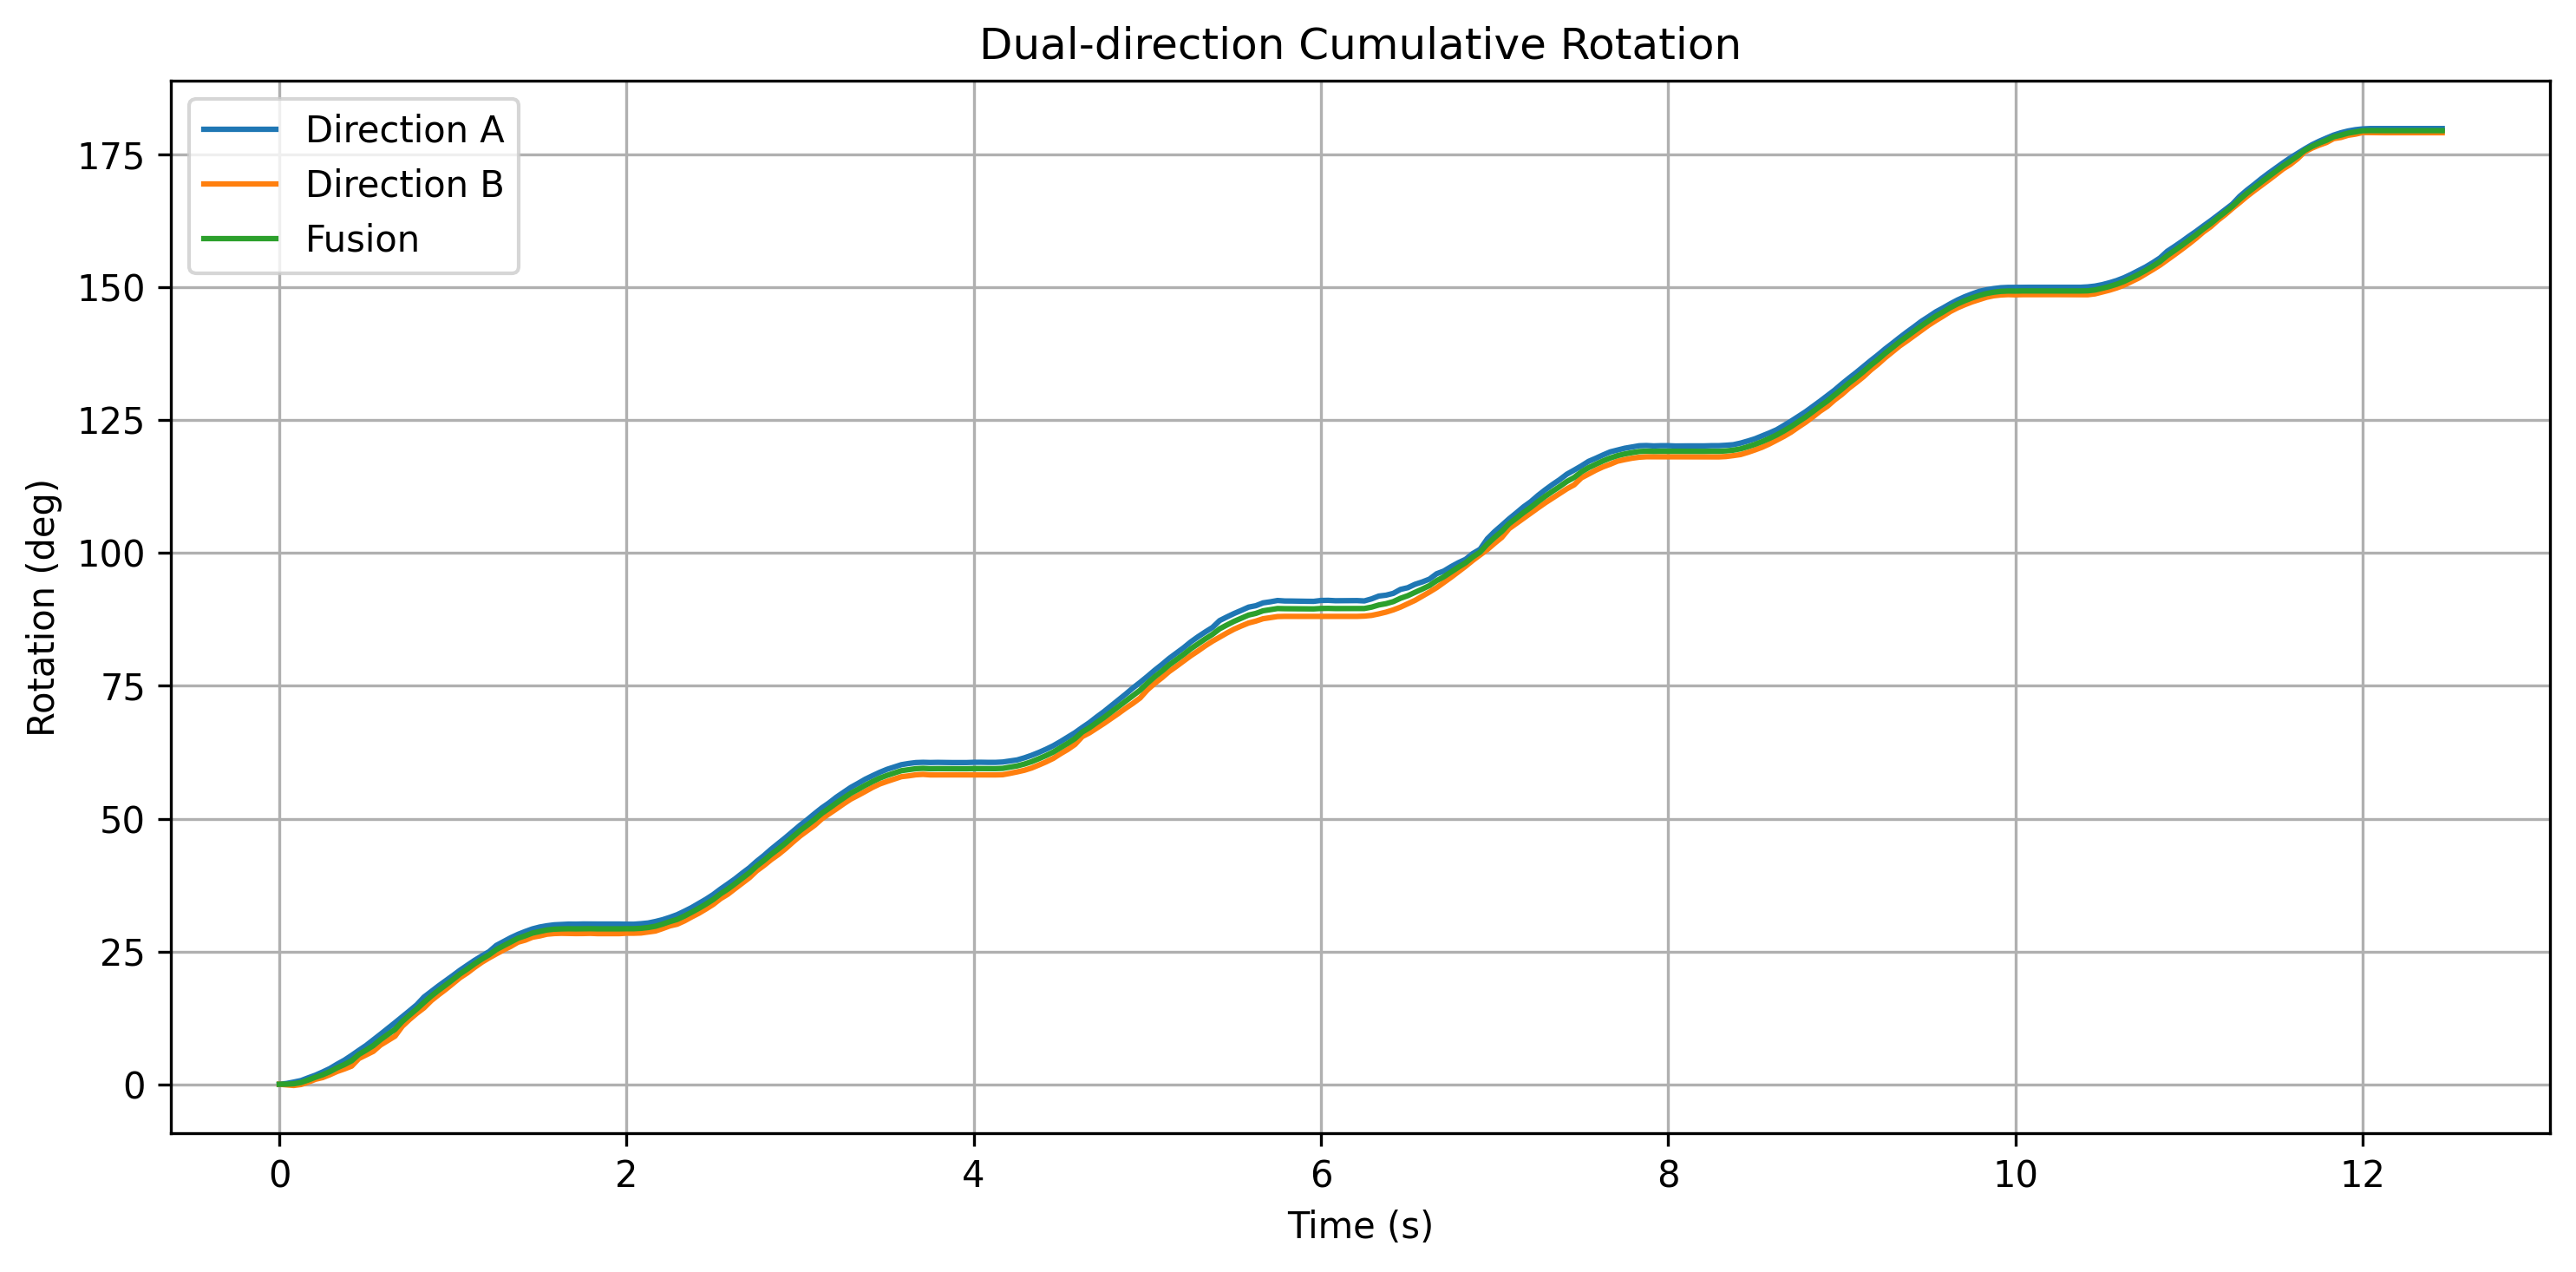
\includegraphics[width=0.8\linewidth]{fig/double_curve.png} 
		\caption{双方向算法角度变化曲线} 
	\end{figure} 
	
	\begin{table}[!htb] 
		\centering 
		\caption{双方向算法检测结果} 
		\begin{tabular}{ccccc} 
			\toprule 
			角度&A&B&平均结果&A/B差值\\ 
			\midrule 
			30&28.33&30.77&29.55&2.45\\ 
			60&58.83&60.63&59.73&1.79\\ 
			90&89.55&89.69&89.62&0.14\\ 
			120&119.70&119.31&119.50&0.39\\ 
			150&149.39&149.77&149.58&0.38\\ 
			180&179.93&179.14&179.53&0.79\\ 
			\bottomrule 
		\end{tabular} 
	\end{table} 
	
	由实验结果可知， 
	双方向算法在不同旋转角度下均能够获得稳定的A/B累计结果。 
	最终融合角度与真实旋转角度保持较小误差， 
	同时A/B方向差值也处于较小范围。 
	
	其中，A/B差值最大为30$^\circ$实验中的2.45$^\circ$， 
	最小为90$^\circ$实验中的0.14$^\circ$。 
	说明不同旋转角度下两个结构方向的检测一致程度存在一定差异， 
	该指标能够为最终角度结果提供额外的可靠性信息。 
	
	\FloatBarrier	% 保证双方向检测结果表格之后，才进入下一节，不会跨页 
	
	\section{算法对比分析} 
	
	\subsection{角度精度对比} 
	
	从实验结果来看， 
	两种算法均能够较好地完成机器人旋转角度估计， 
	但在当前仿真数据上，单方向算法具有更高的数值精度。 
	
	单方向算法的平均绝对误差为0.073$^\circ$， 
	最大误差为0.126$^\circ$； 
	双方向算法的平均绝对误差为0.415$^\circ$， 
	最大误差为0.50$^\circ$。 
	
	因此，在当前规则的Blender仿真环境中， 
	单方向算法在角度数值精度方面表现更好。 
	
	\subsection{稳定性对比} 
	
	单方向算法通过时间连续约束和5帧方向平滑减少帧间方向波动， 
	因此在结构线清晰的情况下具有较好的跟踪稳定性。 
	
	双方向算法则通过A、B两个方向进行相互验证， 
	当两者结果接近时具有较好的一致性， 
	当差值增大时可以提示当前检测可能存在异常。 
	
	因此，单方向算法更突出方向跟踪稳定性， 
	双方向算法则增加了结果一致性的判断能力。 
	
	\subsection{适用场景对比} 
	
	单方向算法结构简单、计算量较低， 
	适合光伏板纹理清晰、结构稳定且主要关注角度精度的场景。 
	
	双方向算法计算过程相对复杂， 
	但能够输出A/B一致性误差， 
	适合需要同时关注角度结果和检测可靠性的场景。 
	
	因此，两种算法并不存在绝对的优劣关系， 
	可根据实际应用对精度、计算量和可靠性的不同要求进行选择。 
	
	\subsection{综合对比} 
	
	\begin{table}[!htb] 
		\centering 
		\caption{两种算法性能比较} 
		\begin{tabular}{ccc} 
			\toprule 
			项目&单方向法&双方向法\\ 
			\midrule 
			方向数量&1&2\\ 
			平均绝对误差&0.073$^\circ$&0.415$^\circ$\\ 
			最大误差&0.126$^\circ$&0.50$^\circ$\\ 
			一致性评价&无&有\\ 
			计算复杂度&低&较高\\ 
			适用重点&角度精度&可靠性评价\\ 
			\bottomrule 
		\end{tabular} 
	\end{table} 
	
	实验结果表明： 
	
	单方向算法由于采用时间连续约束， 
	在当前规则仿真环境下获得了更高角度精度。 
	
	而双方向算法虽然最终误差略高， 
	但能够通过A/B方向差异评价检测结果可靠性， 
	具有更好的结果自检能力。 
	
	综合来看， 
	单方向算法优势在于精度和计算效率， 
	双方向算法优势在于多方向信息融合和可靠性评价。 
	
	\FloatBarrier 
	
	\section{讨论与结论} 
	
	本文研究了基于光伏板结构线方向的机器人旋转角度检测方法。 
	
	实验结果表明， 
	基于光伏板结构线方向的视觉方法能够有效估计机器人旋转角度。 
	
	单方向算法在六组旋转实验中表现出较高检测精度， 
	平均绝对误差为0.073$^\circ$， 
	证明了利用单一结构方向进行累计角度估计的可行性。 
	
	双方向算法进一步利用光伏板正交结构特点， 
	通过A/B方向融合以及一致性误差评价， 
	不仅能够获得旋转角度， 
	还能够对检测结果可靠性进行辅助判断。 
	
	综合来看， 
	单方向算法适合高精度、低计算量的角度估计任务； 
	双方向算法适合需要额外可靠性评价的视觉检测任务。 
	
	需要注意的是，本文实验主要基于Blender仿真环境完成， 
	实际应用中的光照变化、反光、灰尘、遮挡以及纹理缺失等因素， 
	都可能影响LSD直线检测和方向跟踪结果。 
	
	因此未来可以结合： 
	\begin{itemize} 
		\item 光流； 
		\item IMU； 
		\item 特征点跟踪； 
		\item 置信度加权融合。 
	\end{itemize} 
	
	进一步提高复杂环境下机器人旋转角度检测的稳定性和可靠性。 
	
	\appendix 
	\section{算法代码} 
	代码1：单方向累计角度算法。 
	
	代码2：双方向跟踪角度算法。 
	
\end{document}